\chapter{OpenStack}
OpenStack è una piattaforma ideata per la realizzazione e la gestione di infrastrutture cloud complesse, pubbliche e private.
Sviluppato inizialmente da NASA e Rackspace, è oggi amministrato dalla OpenStack Foundation, rilasciato sotto licenza Apache, e sostenuto da aziende del calibro di IBM, Cisco, Citrix, Dell, Oracle e Red Hat.
E' composto da una serie di progetti che si occupano dell'amministrazione delle risorse seguendo il paradigma \textit{infrastructure-as-a-service}; fornisce quindi strumenti per gestire pool di macchine virtuali, lo storage, e le risorse di rete all'interno di un data-center cloud.
Il progetto è open-source ed è interamente realizzato utilizzando il linguaggio Python, seguendo un'architettura totalmente modulare; ogni componente è indipendente dagli altri, e può vivere anche in modalità stand-alone.
I vari produttori solitamente producono delle derivazioni della piattaforma OpenStack, che si differenziano tra loro per la metodologia di automazione del deployment dei componenti e dal parco servizi offerto.
Una di queste metodologie di automazione è rappresentata da DevStack (\textit{http://devstackurl\cite{devstackurl}}), distribuzione di OpenStack orientata allo sviluppo e al testing.
OpenStack è strutturato secondo un approccio multi-tenant, ed offre un livello di astrazione tale da riuscire a garantire molte delle proprietà di sicurezza descritte nel primo capitolo.
I sorgenti sono disponibili nel repository GitHub \textit{https://github.com/openstack/}
\paragraph{}
Nell'ambito del progetto di tesi è stato utilizzato DevStack in configurazione all-in-one\footnote{Tenendo tutti i componenti su un'unica macchina} come riferimento per implementare velocemente alcune delle proprietà di sicurezza su cui sono stati effettuati i test.
In una fase successiva è stato effettuato il deploy manuale di un'infrastruttura più complessa distribuita su cinque nodi.

\section{Componenti di OpenStack}
Tutti i componenti sono implementati come servizi, che espongono delle API REST, invocabili tramite un'interfaccia a riga di comando o la dashboard grafica Horizon.
Grazie alla struttura fortemente modulare e alla natura di software open-source, chiunque può sviluppare un proprio componente seguendo le linee guida della Open Stack Foundation.\cite{GuidelinesOpenstackHacking}
La comunità  OpenStack ha comunque identificato una serie componenti che costituiscono il nucleo dell'intera piattaforma, essi sono considerati parte integrante del progetto e vengono perciò mantenuti ufficialmente dalla comunità OpenStack.
\begin{figure}[H]
\centering
\makebox[\textwidth]{
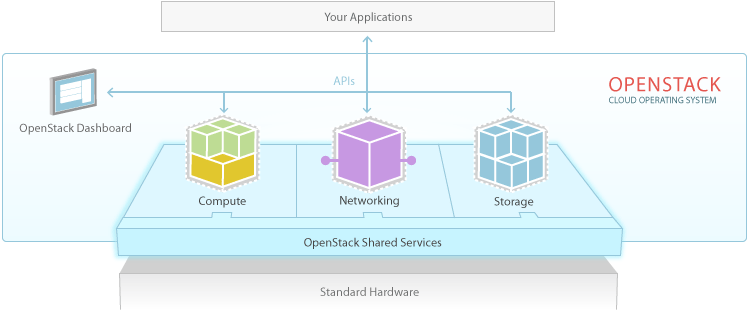
\includegraphics[width=\textwidth]{immagini/openstack-software-diagram.png}
}
\caption{Struttura della Piattaforma Openstack\cite{openstacksoftware}}\label{openstacksw}
\end{figure}
\subsection{Identity service: Keystone}
\textit{Keystone} è il componente di service-catalog, che si occupa anche di fornire i servizi di gestione delle identità, dei token e delle politiche per l'uso specifico dei progetti nella famiglia OpenStack.
E' l'implementazione della Identity API, e ha funzionalità di autenticazione basata su token (authN) e meccanismi di autorizzazione di alto livello (authZ).
E' stato recentemente ristrutturato per essere espandibile e supportare meccanismi AuthN/AuthZ come oAuth, SAML, e openID.
Nella pratica, si occupa di validare le credenziali degli utenti e dei servizi, rilasciare e gestire i token di autenticazione dopo la verifica delle credenziali, e di gestire il catalogo dei servizi tenendo traccia dei relativi endpoint e i livelli di autorizzazione ad essi associati.
Supporta numerosi identity provider di back-end. L'implementazione più comune prevede l'utilizzo di MariaDB per la memorizzazione dei ruoli, delle credenziali e delle sessioni, ma è possibile strutturare architetture federate tramite LDAP o meccanismi di single-sign-on.

\subsubsection{Concetti fondamentali}

\paragraph{Utente}
Rappresentazione digitale di un utente, sistema, servizio che utilizza OpenStack.
Se è un utente ad effettuare la richiesta a Keystone (e l'autenticazione ha esito positivo), il servizio rilascia un token per effettuare le varie richieste.
Gli utenti hanno delle credenziali di login, oppure dei token per accedere alle risorse.
Possono essere direttamente assegnati ad uno o più progetti (\textit{tenant}), che costituiscono un ambiente isolato (\textit{tenant-isolation})
\paragraph{Credenziali}
Dati che confermano l'identità dell'utente (es: nome utente e password, nome utente e chiave API, token di autenticazione)
\paragraph{Autenticazione}
Processo utilizzato per confermare l'identità di un utente, in base alle credenziali fornite.
Una volta avvenuta l'autenticazione, si procede con il rilascio di un token che verrà poi utilizzato per tutte le richieste a seguire.
\paragraph{Token}
Stringa alfanumerica utilizzata per accedere alle API di OpenStack e alle risorse. Può essere revocato in qualunque momento, ed è valido per un periodo definito.
\paragraph{Progetto o tenant}
Un container utilizzato per raggruppare o isolare le risorse. I tenant isolano anche gli oggetti del servizio di identità.
A seconda delle esigenze, potrebbe corrispondere a un cliente, a un'organizzazione o a un progetto.
\paragraph{Servizio}
Un servizio di OpenStack, come Nova, Swift, Glance. Un servizio è caratterizzato da uno o più endpoint, tramite i quali gli utenti possono contattarlo per consultare le risorse da esso custodite ed eseguire le operazioni da esso consentite, nei limiti dei loro privilegi.
\paragraph{Endpoint}
Un indirizzo accessibile via rete per contattare un servizio, solitamente è un URL.
\paragraph{Ruolo}
Una personalità con un insieme definito di privilegi e diritti, su determinate operazioni.
Il token è legato alla lista dei ruoli dell'utente o servizio a cui si riferisce, cosìcche l'utente possa eseguire tutte le operazioni associate all'insieme aggregato dei ruoli a cui appartiene.

\begin{figure}[H]
\centering
\makebox[\textwidth]{
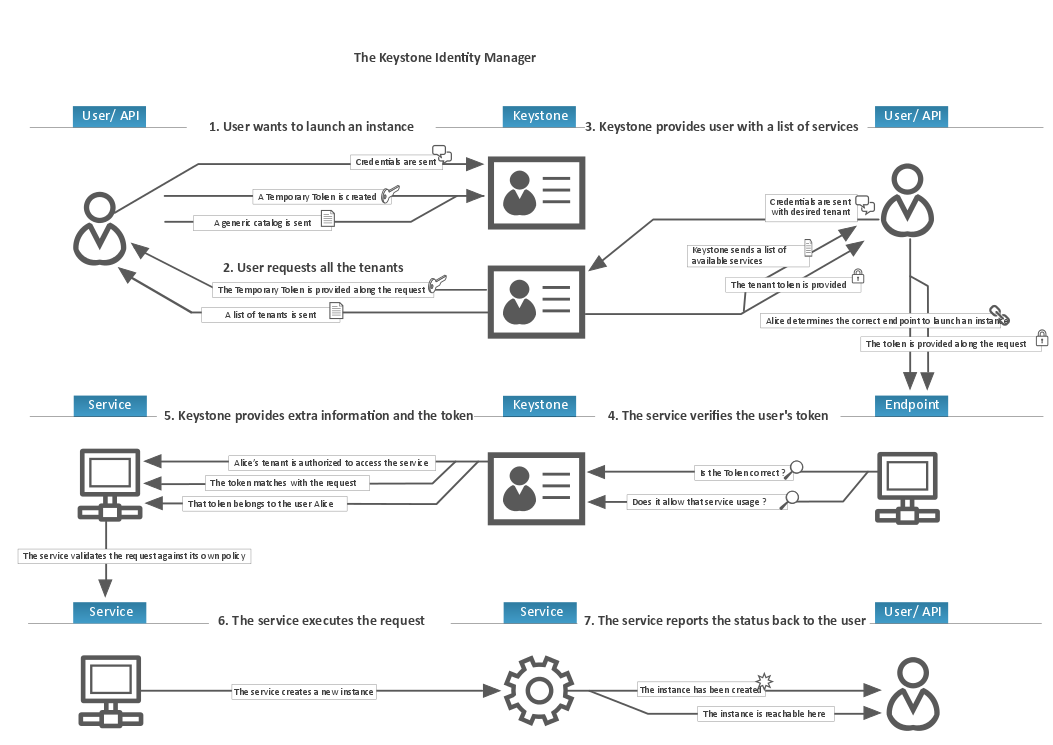
\includegraphics[width=\textwidth]{immagini/KEYSTONE.png}
}
\caption{Diagramma funzionale di Keystone\cite{openstackkeystone}}\label{openstackkeystone}
\end{figure}

\subsection{Compute service: Nova}
\textit{Nova} è il componente che si occupa di gestire la parte di Compute di OpenStack. La sua architettura è progettata in un'ottica di scalabilità orizzontale e poggia le sue basi sulle tecnologie di virtualizzazione note. Come hypervisor di backend, infatti, può fare uso di KVM, Xen Server, VMware ed altri.
Le sue funzionalità sono suddivise in vari servizi:
\begin{itemize}
\item \textbf{nova-api}: servizio che si occupa di gestire le richieste di allocazione e gestione delle risorse computazionali effettuate dagli utenti.
Costituisce il cuore dell'interno framework e fornisce la possibilità di controllare l'hypervisor, lo storage e le funzionalità di rete.
Gli endpoint sono servizi HTTP che gestiscono le varie funzioni utilizzando vari tipi di interfaccia (Amazon, Rackspace) e i relativi modelli. Ciò permette alle API di interagire con strumenti già esistenti creati da altri provider.
In un'architettura multi-nodo questo servizio viene installato ed eseguito sul nodo \textit{Controller}.
\item \textbf{nova-scheduler}: si occupa di effettuare lo scheduling delle operazioni invocate da nova-api. Funziona per mezzo di una coda, ed è in grado di individuare il nodo di Compute sul quale deve essere effettuato il deploy delle varie istanze virtuali. Aggiunge dunque un livello di astrazione al fine di consentire la scalabilità orizzontale. Anche questo servizio, nel caso di setup multi-nodo, viene eseguito sul nodo \textit{Controller}.
\item \textbf{Coda di messaggi}, attraverso la quale è orchestrata l'interazione tra i nodi di compute, il controller di rete, le API, lo scheduler e gli altri componenti.
I vari worker leggono cosantemente la coda in base al loro ruolo o, per esigenze specifiche, al loro hostname.
Quando arriva un task sulla coda, il worker ad esso demandato lo esegue e rimanda indietro la risposta, portando il feedback all'utente o servizio che ha generato la richiesta iniziale.
\item \textbf{nova-compute}: è un worker che interagisce con le API dell'hypervisor per creare, eliminare, modificare le varie istanze e le risorse ad esse assegnate. Questo servizio viene generalmente eseguito sullo stesso nodo dell'hypervisor.
Si occupa di:
\begin{itemize}
\item Avviare istanze
\item Terminare istanze
\item Riavviare istanze
\item Agganciare un volume a un'istanza
\item Sganciare un volume da un'istanza
\item Ottenere l'output della console
\end{itemize}
\item \textbf{nova-network}: è il controller di rete. Si occupa principalmente di amministrare le risorse di rete sui vari host. Si occupa di:
\begin{itemize}
\item Allocare indirizzi IP fissi
\item Configurare le VLAN dei vari progetti o tenant
\item Configurare la rete sui nodi di compute
\end{itemize}
Nelle release più recenti di Openstack, \textit{nova-network} è stato sostituito da un servizio dedicato: \textit{neutron}.
\item \textbf{nova-rootwrap}: consente di interagire con le API dell'hypervisor in modo sicuro, senza essere \textit{root} sulla macchina dell'hypervisor, sostituendo il comando \textit{sudo}.
\item \textbf{nova-consoleauth, nova-novncproxy, nova-xvpvncproxy}: si occupano di fornire l'accesso KVM\footnote{Keyboard, Video, Mouse} per le macchine virtuali. Solitamente, affinché ciò possa avvenire, sono utilizzati protocolli di desktop remoto come VNC, Spice, o RDP, a seconda di quanto supportato dall'hypervisor.
Il deploy di questi servizi avviene generalmente in questo modo
\begin{itemize}
\item Un processo \textit{nova-consoleauth} sul nodo controller.
\item Un processo \textit{nova-novncproxy} o \textit{nova-xvpvncproxy} sullo stesso nodo delle \textit{nova-api} (spesso nodo Controller). La differenza tra i due, è che il primo fa uso di un client basato su HTML5, mentre l'altro sfrutta la tecnologia Java. 
\end{itemize}
Le connessioni alla console, sia che siano fatte in modo diretto, sia attraverso un proxy, passano attraverso le porte TCP comprese tra 5900 e 5999. Il firewall di ogni nodo di compute deve perciò avere la seguente regola:
\begin{python}
-A INPUT -p tcp -m multiport --dports 5900:5999 -j ACCEPT
\end{python}
\end{itemize}

\begin{figure}[H]
\centering
\makebox[\textwidth]{
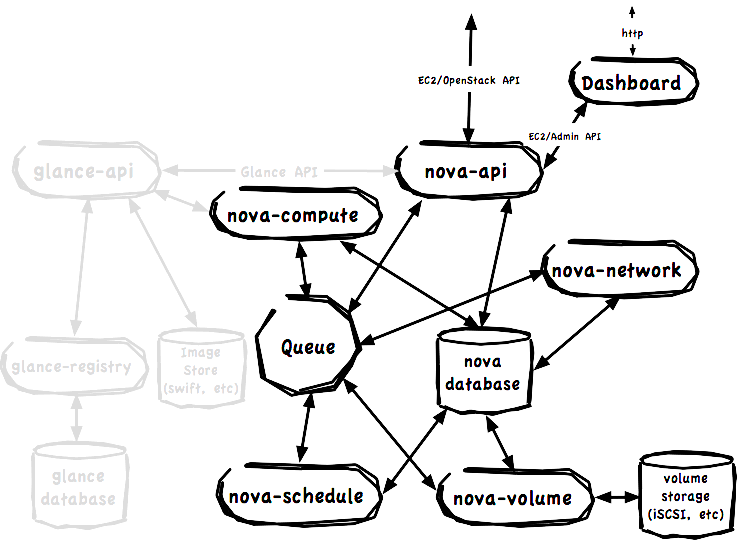
\includegraphics[width=\textwidth]{immagini/nova.png}
}
\caption{Diagramma funzionale di Nova\cite{openstacknova}}\label{openstacknova}
\end{figure}

\subsection{Image service: Glance}
\textit{Glance} si occupa della conservazione e la registrazione delle immagini di base per istanziare nuove macchine virtuali.
Il servizio espone un'interfaccia REST che consente di:
\begin{itemize}
\item reperire i metadati relativi a un'immagine
\item caricare una nuova immagine, e registrare i relativi metadati
\item scaricare un'immagine in locale
\end{itemize}
Glance fornisce la possibilità di memorizzare le immagini in varie locazioni. Esse possono infatti essere dei semplici file sul disco fisso del nodo su cui Glance è stato eseguito, oppure altri tipi di storage come Swift (il servizio di object-storage).
Esso è scritto secondo i seguenti principi:
\begin{itemize}
\item Architettura componibile
\item Alta disponibilità e scalabilità
\item Tolleranza ai guasti
\item Recuperabilità
\item Utilizzo di tecnologie standard aperte
\end{itemize}

\subsection{Networking service: Neutron}
\textit{Neutron} è il componente di OpenStack che offre il servizio di "networking as a service" per le macchine virtuali, effettuando un'astrazione del livello di rete.
Lo scopo è principalmente quello di fornire delle API per strutturare la rete in modo avanzato e costruire topologie complesse, dotate di politiche di networking eterogenee.
Affinché ciò possa avvenire, Neutron fa uso di tecnologie di software-defined networking, come OpenFlow e Open-vSwitch, incapsulando il traffico con varie tecnologie di tunneling come VXLAN e GRE.
E' strutturato su un'architettura totalmente componibile tramite plug-in, che possono essere sia open-source che proprietari, i quali forniscono le modalità per amministrare in modo efficiente le capabilities di rete.
La filosofia è quindi quella di implementare l'approccio \textit{as-a-service} anche per il livello di rete, al fine di fornire le seguenti funzionalità:
\begin{itemize}
\item Load balancer-aaS
\item VPN\footnote{Virtual Private Network}-aaS
\item Firewall-aaS
\item IDS-aaS
\item etc.
\end{itemize}
Un'altra funzionalità introdotta da Neutron, è quella di creare molteplici reti virtuali e di garantire la tenancy isolation agendo direttamente sul livello 2 dello stack ISO/OSI
Le API forniscono inoltre numerosi livelli di controllo per:
\begin{itemize}
\item Politiche di sicurezza e \textit{compliance}
\item Qualità del servizio
\item Monitoraggio e risoluzione dei problemi
\end{itemize}

%http://www.slideshare.net/danwent/openstack-quantum-intro-os-meetup-32612

\begin{table}[h]
\centering
\begin{tabular}{| m{3cm}| m{5cm} | m{5cm} | }
\hline
& \textbf{Nova} & \textbf{Neutron} \\ \hline
\textit{*-as-a-service} & Compute & Network \\ \hline
\textit{Livello di astrazione} & \textbf{server virtuali}, rappresentano host con una CPU, della RAM, dischi, e interfacce di rete & \textbf{reti virtuali}: segmenti di livello 2, \textbf{porte virtuali}: punti di aggancio per i dispositivi connessi alle reti virtuali \\ \hline
\textit{Tecnologie di backend supportate} & libvirt per KVM, XenServer, Hyper-V, vMware ESX & Open vSwitch, Cisco UCS, Linux Bridge \\ \hline
\textit{Espandibilità delle API} & \textit{keypair}, ripristino delle istanze, volumi, etc. & \textit{QoS}, statistiche sulle porte, \textit{security groups}, etc. \\ \hline

\end{tabular}
\caption{Analogie tra Neutron e Nova}
\label{tab:AnalogiesNeutronNova}
\end{table}
\begin{figure}[H]
\centering
\makebox[\textwidth]{
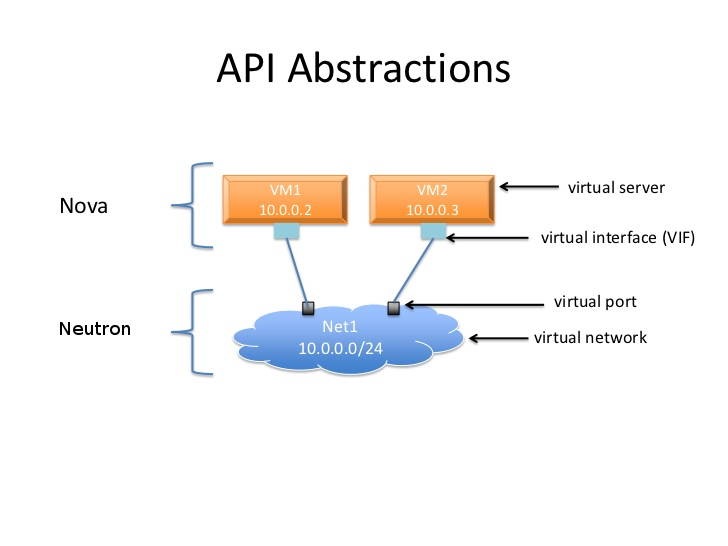
\includegraphics[width=\textwidth]{immagini/neutronNova.jpg}
}
\caption{\cite{NeutronNova}}\label{NeutronNova}
\end{figure}

\subsection{Object-storage service: Swift}

\subsection{Block-storage service: Cinder}

\subsection{Altri servizi} 
\subsubsection{Database service: Trove}
\subsubsection{Orchestration service: Heat}
\subsubsection{Bare-metal service: Ironic}
\subsubsection{Data-processing service: Sahara}
\subsubsection{Messaging service: Zaqar}
\subsubsection{Key management service: Barbican}
\subsubsection{DNS service: Designate}
\subsubsection{Shared Filesystem service: Manila}
\subsubsection{Application catalog service: Murano}
\subsubsection{Governance service: Congress}
\subsubsection{Workflow service: Mistral}
\subsubsection{Key-value store \textit{as-a-service}: MagnetoDB}

\section{Servizi di supporto}
\subsection{Dashboard: Horizon}
\subsection{Telemetry-service: Ceilometer}
\subsection{Benchmark-service: Rally}
\subsection{API Testing: Tempest}
\section{Deploy di OpenStack con DevStack}
\subsection{Devstack e SSL}
\section{Sicurezza e certificazione di OpenStack}